\begin{document}
	
	\subsection{Training}
	
	This step consist in the estimation of the centroids of the color space. May be  really time consuming, but it is performed only once, so during the actual segmentation the corresponding script isn't run.\\
	To achieved the estimation of centroids, a k-means clustering of the multichannel images of several CT scan from different patients is performed. 
	In order to achieve a uniform representation of each cluster, the scans included in the training set were carefully selected from the $3$ datasets used in this work. The main rule used for the selection is that in each scan must me present a huge amount of infection areas and also a well representation of artifacts, in order to takes into account all the possible features.\\
	The achievement of the training task involves two main steps : 
	\begin{enumerate}
		\item \textbf{Preparation of images} : involves the building of the multi channel images, and the registration in a common space; 
		
		\item \textbf{Clustering} : Actual clustering, involves also the managing of the background problem.
	\end{enumerate}

		\subsubsection*{Preparation of Images} 
	
		This step involves the preparation of images, with the building of the multi channel image that incorporates neighbouring and edges information as well as the registration in a common space and the managing of an allocation memory problem.\\
			
		As I've said the multichannel image is build to incorporate more information during the clustering. We have found that a 4 channel image will provides good segmentation results. The 4 channel of the image are built as follows  : 
		\begin{itemize}
			\item Pure image after histogram equalization; 
			\item Median Blurring of the equalized image; 
			\item Gamma corrected image;
			\item Standard filtered image.
		\end{itemize}
	
		\begin{figure}[h]
			\centering
				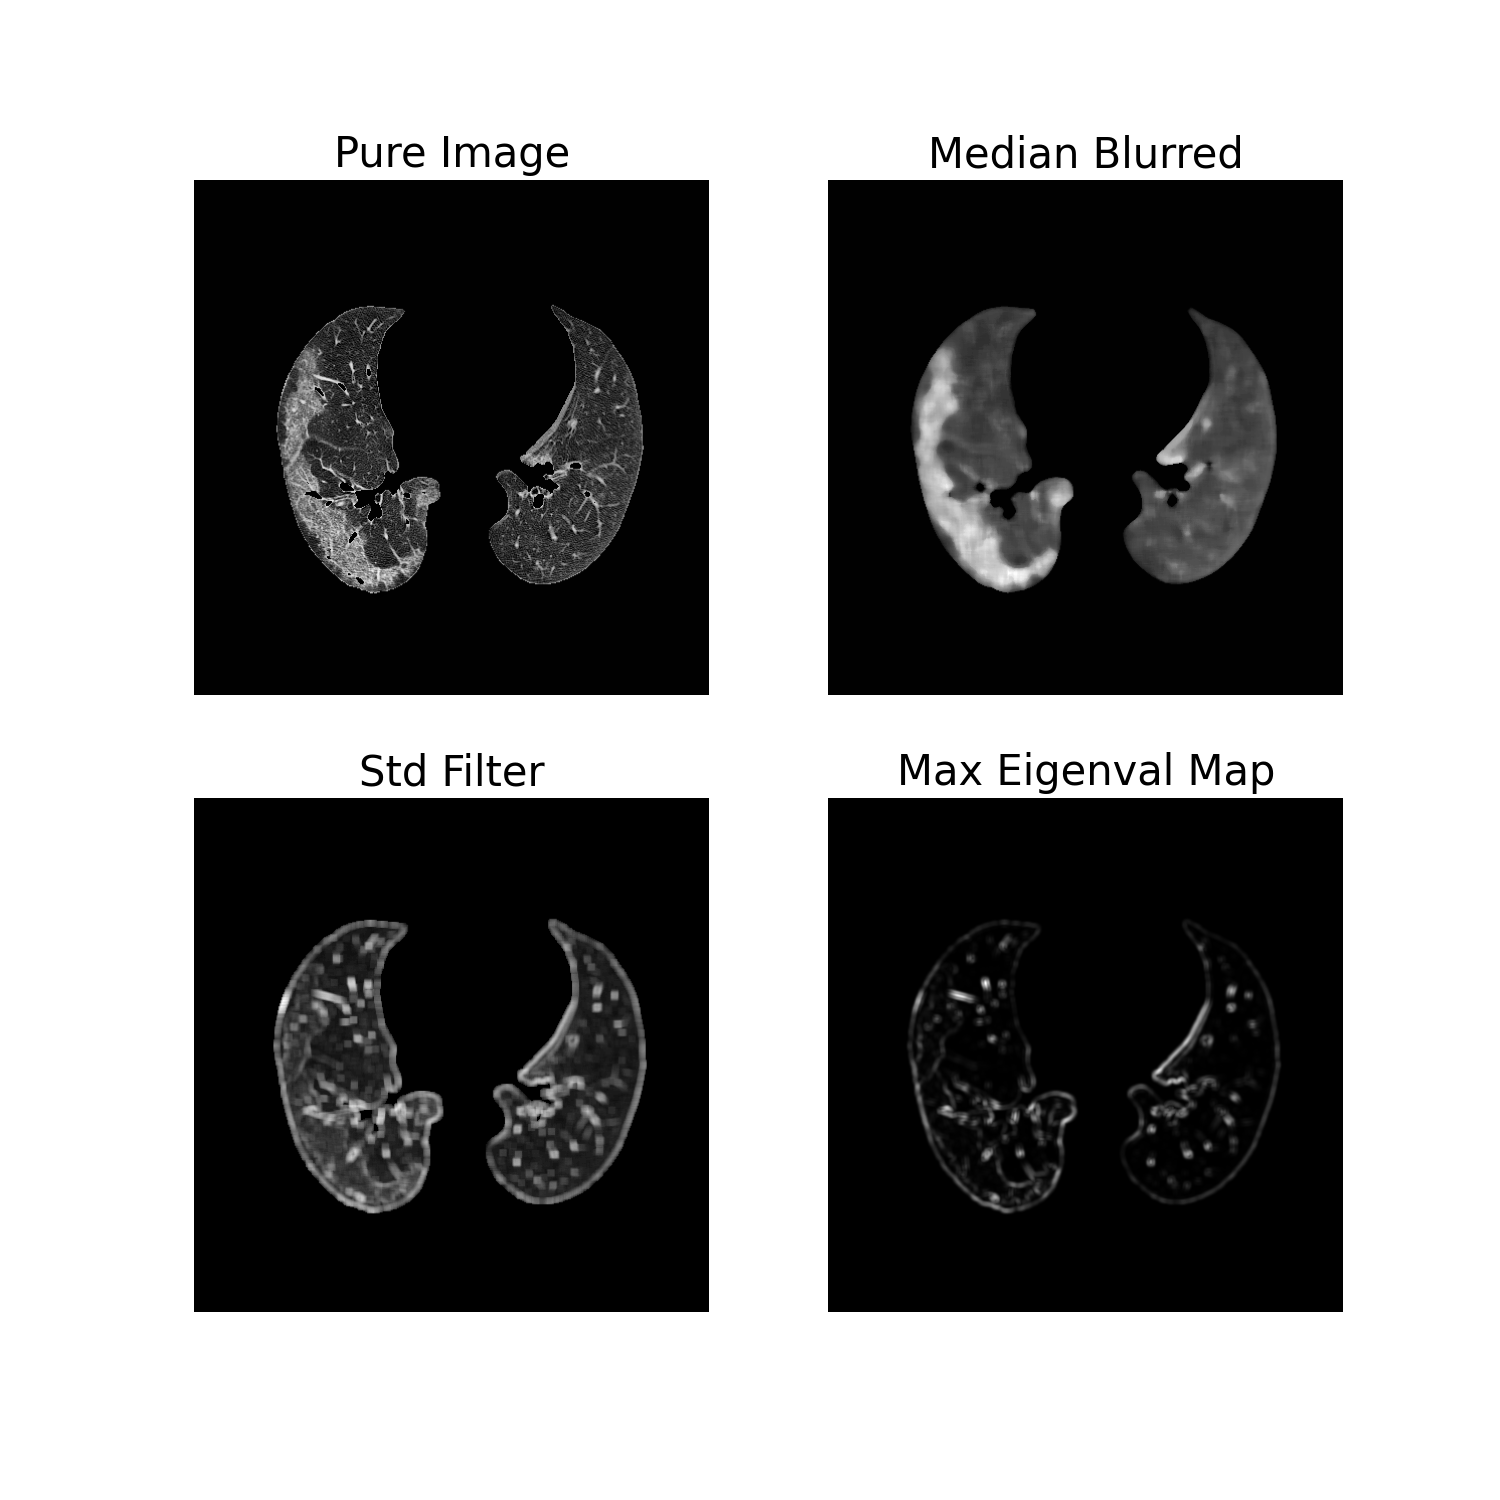
\includegraphics[scale=.55]{Multi_Channel.png}
			\caption{Channels of the image. From left to right and from top to bottom the imageaffter the histogram equalization, the gamma corrected image, the median blurred image and the std fitered image. This channels allow us to consider informations about the single voxel but also about the neighbouring voxels and their variability. }\label{fig:MultiChannel}
		\end{figure}
	
		In \figurename\,\ref{fig:MultiChannel} I've displayed the 4 different channel of the image. Each channel allow us to consider different information\\
		The histogram equalized image and the gamma corrected allows to takes into account information about the single voxel. The histogram equalization is applied in order to ehance the image contrast by improving the GL usage. For each slice the histogram is equalized operating in small image regions, in order to takes care of the over-amplification of the contrast.
		
		 The gamma correction is a non linear operation and is used to decode the luminance, and to made in evidence the less evident lesions. Both of this filters involves the single voxel.\\The median blurring allow us to consider also the information of the neighborhood voxels, allowing the reduction of the outliers. The usage of this filter is justified since the lesions involves several closest voxels.
		 
		 The last channel used is the image after the application of a local standard deviation filter which consist in the replacement of each pixel value with the standard deviation of its neighborhood, help us to distinguish the remaining bronchial and artifact structures.
		
		Each image channel is normalized according to means and standard deviation of the whole scan.
		
		The first step consist into the construction of the multichannel image of for each input series, after that all the images are shuffled and divided into several sub-samples. If the provided training dataset is huge, may happen that the required memory cannot be allocated. Divide the training set into several subsamples lead to less memory requirement, allowing the training. From this step we obtain a several set of centroids, on whoch a second clustering is performed, in order to found the final centroid matrix.
		
		
		The creation of several sub-samples is made since the creation of a single, huge array with several images is not always possible, since requires a huge quantity of memory to be allocated, so we have chose to divide all the images into several sub-samples and cluster them independently, after that a clustering on the estimated centroids is performed.\\

		
		\subsubsection*{Clustering} 
		
		This step consist into the performing of the k-means clustering for the centroids estimation. To perform this task I've used the OpenCV algorithm, which provides an optimized implementation of the algorithm for multi channel images. A first clustering is applied on each sub-sample, resulting in a set of centroids for each one of them. On this set is applied a second clustering, which provides the actual centroids. In both of the clustering, the initial centroids set is initialized by using the k-means ++ algorithm, which allows to improve speed and accuracy of the clustering algorithm~\cite{Arthur2007}.
		
		During this task we have to manage some issues. As we can see from \figurename\,\ref{fig:ClusteringHistogram} the number of voxel with $GL = 0$  is several order of magnitude higher than for other $GL$. As prior we know that these voxels belonging from background, so this cluster is over represented. Since kmeans cluster requires an homogeneous representation for each cluster, this may raise problem during the centroids estimation. In order to overcome this issue we have simply removed this voxels from the clustering.  
		

		\begin{figure}[h!]
			\centering
				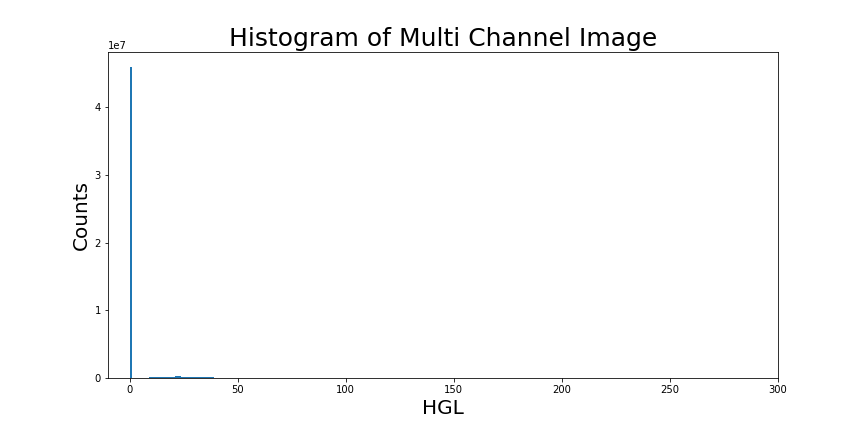
\includegraphics[scale=.32]{HistMC.png}
				\caption{Histogram of the multichannel image to cluster, we can clearly see the overrepresented cluster at $0$ GL}	\label{fig:ClusteringHistogram}
		\end{figure}
		
	An other problem may be the estimation of the correct number of clusters. k-means clustering requires a prior knowledge on the number of clusters which is a crucial choice. In our case the anatomical knowledge about the lung may help, since we can consider one cluster for each anatomical structure. In the end we have found that 5 clusters are an optimal choice, and the considered structures are the following: 
	\begin{itemize}
		\item Lung Parenchima;
		
		\item Edges;
		
		\item vessel surrounding bronchial structures;
		
		\item Ground Glass Opacities and consolidation;
		
		\item Bronchi.

	\end{itemize}

	
	We don't need a cluster to represent the background, since as I' ve said before the corresponding voxel aren't takes into account during the clustering.\\
	In the end a set of centroids for each subsamples was estimated and a second clustering was performed, to found the optimal centroids. 
	This process takes a lot of time, but once we have estimated the optimal centroid set, we haven't to repeat it.\\
	
	The whole step is summarized in the pseudocode in \figurename\,\ref{alg:training}.
		
		
	\begin{algorithm}
	
	\SetAlgoLined
	\DontPrintSemicolon
	
	\KwData{CT scans with Extracted lung}
	\KwResult{Centroid matrix}\;
	
	\ForEach{$scan \in input\_scans$}{
	
		read the scan\;
		sample$\leftarrow$image\_array\;
	}\;
	\tcc{prepare subsamples}
	sample$\leftarrow$ build\_multichannel(sample)\;
	sample$\leftarrow$shuffle(sample)\;
	subsamples$\leftarrow$split(sample)\;
	
	\tcc{start the first clustering}
	\ForEach{$ Sub \in subsamples $}
	{
		center$\leftarrow$kmeans(sub, number of centroids)\;
		centroid\_vector$\leftarrow$append(center)
		
	}\;

	\tcc{Refinement}
	centroid\_matrix$\leftarrow$kmeans\_clustering(centroid\_vector, n\_centroids)\;
	
	\caption{Pseudo-code for the training script}\label{alg:training}
	
\end{algorithm}

	
\end{document}